%!TEX root = ../main.tex

%=============================================================================== 
%
%    Chapter: math_fundamentals
%
%=============================================================================== 

\chapter{Math fundamentals}
\label{chapter:math_fundamentals}

In this chapter we'll review the fundamental ideas of mathematics, including numbers, equations, and functions.  
To understand college-level textbooks, you need to be comfortable with mathematical calculations.
Many people have trouble with math, however. 
Some people say they \emph{hate} math, or could never learn it. 
It's not uncommon for children who score poorly on their school math exams to develop math complexes in their grown lives.
If you are carrying any such emotional baggage, you can drop it right here and right now.

Do NOT worry about math! 
You are an adult, and you can learn math much more easily than when you were a kid.
We'll review \emph{everything} you need to know about high school math, and by the end of this chapter, 
you'll see that math is nothing to worry about.

\smallskip

\begin{figure}[H]
\centering
\! 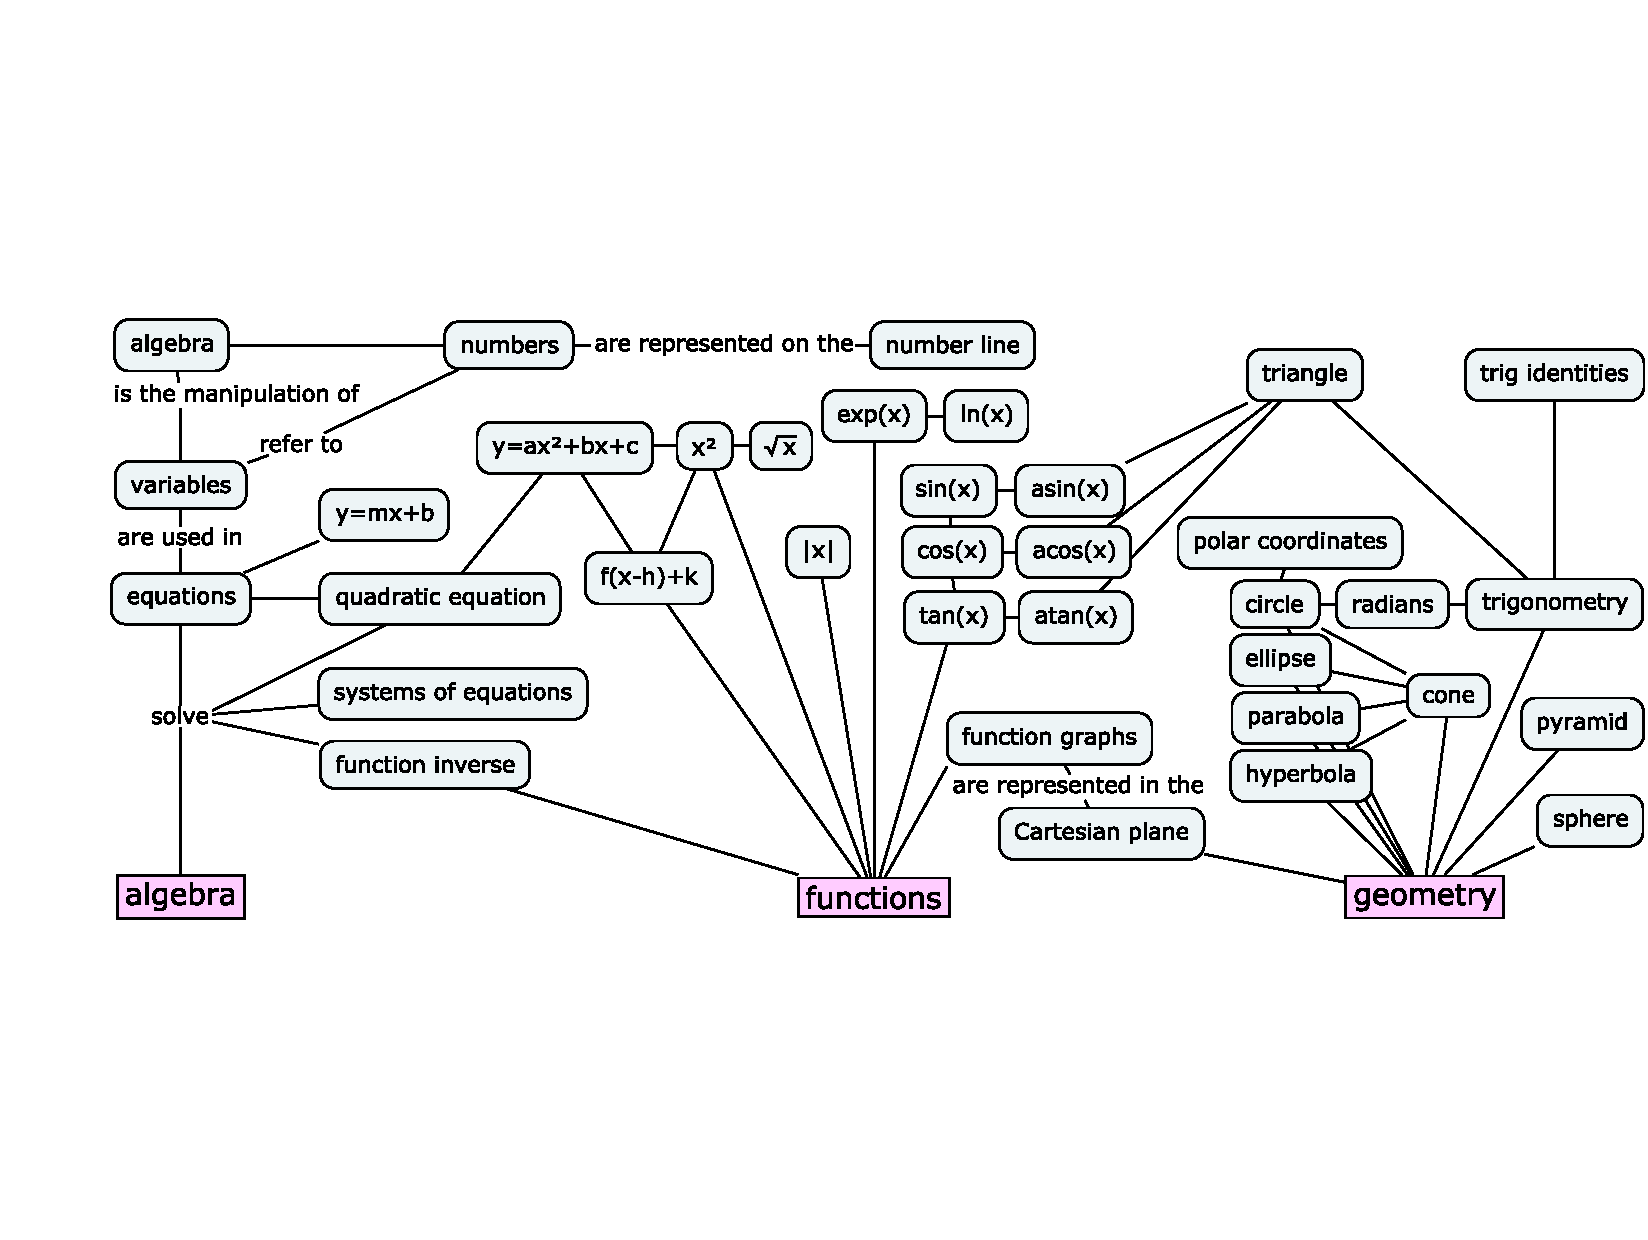
\includegraphics[width=1.01\textwidth]{figures/concept_maps/precalculus.pdf}
	\caption{A concept map showing the mathematical topics that we will cover in this chapter.
			We'll learn how to solve equations using algebra, 
			how to model the world using functions,
			and how to think geometrically.
			The material in this chapter is required for your understanding of the more advanced topics in this book.}
\label{fig:precalculus_concept_map}
\end{figure}
